\documentclass[11pt,fleqn]{exam}
\usepackage[utf8]{inputenc}
\usepackage[T1]{fontenc}
\usepackage{fancyvrb}
\usepackage{amsmath}
\usepackage{amssymb}
\usepackage{hyperref}
\usepackage{algpseudocode}
\usepackage{comment}
\usepackage{enumitem}
\usepackage[margin=0.75in]{geometry}
\usepackage{tikz}
\usetikzlibrary{arrows,arrows.meta,positioning,intersections,shapes.gates.logic.US,calc}
\algnewcommand\algorithmicforeach{\textbf{for each}}
\algdef{S}[FOR]{ForEach}[1]{\algorithmicforeach\ #1\ \algorithmicdo}
\newcommand{\fillinMCmath}[1]{
\begin{tikzpicture}\draw circle [radius=0.5em];\end{tikzpicture}\ #1}
\newcommand{\fillinMCmathsoln}[1]{
\begin{tikzpicture}\draw[black, fill=blue] circle [radius=0.5em];\end{tikzpicture}\ #1}
\newcommand{\ptsamt}[1]{[#1~points]}
\newcommand{\ptamt}[1]{[#1~point]}

%%% Adding Colour to Questions and Answers
\usepackage{color}

\definecolor{solnblue}{rgb}{0,0,1}
\newenvironment{soln}{\color{solnblue}}{}

%Questions

% Answers
\definecolor{blu}{rgb}{0,0,0.5}
\def\blu#1{{\color{blu}#1}}
\definecolor{gre}{rgb}{0,.3,0}
\def\gre#1{{\color{gre}#1}}
\definecolor{red}{rgb}{0.5,0.0,0}
\def\red#1{{\color{red}#1}}
\def\norm#1{\|#1\|}
%%% End for Colours

\bracketedpoints

\makeatletter
\renewenvironment{solution}{\leavevmode\par\begin{soln}\noindent Solution:}{\end{soln}}
\makeatother
      \newif\ifsolutions\solutionsfalse

\author{}
\date{}
\title{CPSC 320 2025S: Assignment 1}

\begin{document}
	
	\maketitle
	\vspace{-0.5in} This assignment is due \textbf{Friday, July 11 at 7 PM}. Late submissions will not be accepted. Please follow these guidelines:
	\begin{itemize}
		\item Prepare your  solution using \LaTeX \ and submit  a pdf file. Easiest will be to submit using
		the .tex file provided. For questions where you  need to select a circle, you can simply
		change \verb~\fillinMCmath~ to \verb~\fillinMCmathsoln~ .
		
		\item Enclose each paragraph of your solution with
		\verb~\begin{soln}Your solution here...\end{soln}~.
		\begin{soln}Your  solution will  then appear  in dark  blue\end{soln}, making  it a  lot
		easier for TAs to find what you wrote.
		
		\item   Submit   the    assignment   via   \href{https://gradescope.ca/}{GradeScope}. You will be get access to Gradescope on the 9th of July via an invite link. Your group must make  a \textbf{single} submission via one
		group member's account, marking all other group members in that submission \textbf{using
			GradeScope's interface}.
		
		\item  After uploading  to  Gradescope, link  each  question  with the  page  of your  pdf
		containing your solution. 
	\end{itemize}
	
	Before we  begin, a few  notes on pseudocode throughout  CPSC 320: Your  pseudocode should
	communicate your algorithm  clearly, concisely, correctly, and  without irrelevant detail.
	Reasonable use  of plain  English is  fine in  such pseudocode.  You should  envision your
	audience as a capable CPSC 320 student unfamiliar with the problem you are solving. You may \textbf{neither} include what we consider to be irrelevant coding details \textbf{nor} assume that  we understand the particular  language you
	chose. (So, for example,  do not write \texttt{\#include <iostream>} at  the start of your
	pseudocode,   and    avoid   language-specific   notation   like    C/C++/Java's   ternary
	(question-mark-colon) operator.)
	
	Remember also  to \textbf{justify/explain  your answers}. We  understand that  gauging how
	much  justification to  provide can  be tricky.  Inevitably, judgment  is applied  by both
	student and  grader as to how  much is enough, or  too much, and it's  frustrating for all
	concerned  when judgments  don't align.  Justifications/explanations need  not be  long or
	formal, but  should be  clear and  specific (referring  back to  lines of  pseudocode, for
	example). Proofs should be a bit more formal.
	
	On the  plus side, if  you choose an  incorrect answer when  selecting an option  but your
	reasoning shows partial  understanding, you might get more marks  than if no justification
	is provided. And  the effort you expend  in writing down the  justification will hopefully
	help you gain deeper  understanding and may well help you converge  to the right selection
	:).
	
	\vspace{.1in}
	
	Ok, time to get started...
	
	\clearpage
	
	\section*{Group Members}
	
	Please list the CWLs of all group members here (even if you are submitting by yourself). We will deduct a mark if this is incorrect or missing.
 
	\section{Tiles and Tribulations}

You're given a grid of size $n \times n$, where $n = 2^k$ for some $k \ge 1$, with one cell missing. Your job is to cover the board with \textit{L-tiles}. An L-tile is three squares that form an L shape (i.e., a $2\times 2$ square with one square missing). Below is a $4 \times 4$ board, with a missing cell at position $(2,3)$ (using 1-based indexing from bottom left).

\begin{figure}[tbh!]
	\centering
	\includegraphics[width=0.6\columnwidth]{a4-tiles.pdf}
\end{figure}

The L-tiles:
\begin{itemize}
	\item Must cover every white square of the board.
	\item Must NOT cover the single black square on the board.
	\item Are not allowed to overlap.
\end{itemize}

\begin{questions}
	\question[5] Prove that, for any $2^k \times 2^k$ board with an arbitrary missing cell, we can come up with a way to cover the board with L-tiles. (Hint: induction on $k$ works well.)

	\begin{soln}
		For a \(2^1 \times 2^1\) board we can cover the board using one \(L-tile\) by removing any arbitrary square, thus our base case \(n = 1\) holds.

		Assume that we can cover any \(2^k \times 2^k\) board using \(L\)-tiles when a square is missing with \(k \geq 1\).

		Now consider a \(2^{k+1} \times 2^{k+1}\) board with an arbitrary missing square.

		We partition this \(2^{k+1} \times 2^{k+1}\) board into four \(2^k \times 2^k\) quadrants, each of which maintains the structure of a square. We label them \(Q_1, Q_2, Q_3, Q_4\) using traditional convention that \(Q_1\) is top-right quadrant and so forth.

		The removed cell must appear in at least one of these sections. By the inductive hypothesis, we can cover it using \(L-tiles\).

		WLOG, assume the missing cell is in top-right quadrant, \(Q_1\). If not, we can rotate our board and relabel the quadrants accordingly.

		Then observe that the bottom-right square of \(Q_2\), the top-right square of \(Q_3\), and the top-left square of \(Q_4\) forms an \(L-tile\).

		Remove these cells from the respective quadrants and we get that by the inductive hypothesis we can cover those qudrants using \(L-tiles\).

		Return the cells using the described \(L-tile\) and we get that we can cover the \(2^{k+1} \times 2^{k+1}\) board using \(L-tiles\) with a square missing.

	\end{soln}


	\ifsolutions\input{q1a-sol.tex}\fi

	\question[5] Design a divide-and-conquer algorithm to place L-tiles to cover a $2^k \times 2^k$ board with a single missing cell.

		\begin{soln}
     \(B\) can be thought of as an \( n \times n \) matrix where \( n = 2^k \) for some integer \( k \geq 1 \). The matrix represents a square board. 

      For ease of notation we may also say \(B = \{(i, j) : 1 \leq i, j \leq n\}\).

      The coordinate \((1, 1)\) refers to the bottom-left corner of the board, in particualar it's the origin.

      For \((i, j)\), first coordinate denotes horizontal position, second coordinate denotes vertical position.

      The solution \( S \) is defined as a collection of sets of coordinates \( \{L_1, L_2, \dots, L_m\} \), where each \( L_i \) is a set of three coordinates that together form an \( L \)-shape.

      We say that \(L_i\) is an \(L-shape\) if each of its coordinates are adjacent to each other and they do not form a \(3-cell\) line.

      Additionally, the sets must satisfy the following conditions, where \((x, y)\) is the missing cell:
    \[
      \bigcap_{i=1}^{m} L_i = \varnothing \quad \text{(pairwise disjoint)}, \quad \text{and} \quad \bigcup_{i=1}^{m} L_i = B \setminus \{(x, y)\} \quad \text{(fully covers the board)}.
    \]

			\begin{algorithmic}[1]
        \Procedure{Cover-Board}{$B$, $n$, $(x, y)$}
        \If {$n = 2$}
        \State \Return {$B \setminus \{(x, y)\}$}
        \EndIf
        \State $B_1 \gets \text{First Qaudrant of } B$ 
        \State $B_2 \gets \text{Second Qaudrant of } B$ 
        \State $B_3 \gets \text{Third Qaudrant of } B$ 
        \State $B_4 \gets \text{Fourth Qaudrant of } B$ 

        \State $L \gets$ Middle square coordinates

        \State Identify $l \in \{1, 2, 3, 4\}$ such that {$(x, y) \in B_l$}
        \State $L := L \setminus B_l$

        \State $L' \gets L \cup \{(x, y)\}$

        \State $B_1 = \text{Cover-Board($B_1$, $\frac{n}{2}$, $B_1 \cap L$)} $
        \State $B_2 = \text{Cover-Board($B_2$, $\frac{n}{2}$, $B_2 \cap L$)} $
        \State $B_3 = \text{Cover-Board($B_3$, $\frac{n}{2}$, $B_3 \cap L$)} $
        \State $B_4 = \text{Cover-Board($B_4$, $\frac{n}{2}$, $B_4 \cap L$)} $
        \State \Return $B_1 \cup B_2 \cup B_3 \cup B_4 \cup L$
				\EndProcedure
			\end{algorithmic}

			\begin{algorithmic}[1]
				\Procedure{Wrapper-Call}{$B$, $n$, $(x, y)$}
        \State \Return \text{Cover-Board}($B$, $n$, $(x, y)$)
				\EndProcedure
			\end{algorithmic}

	\end{soln}

	\ifsolutions\input{q1b-sol.tex}\fi

	\question[2] Give and briefly justify a good asymptotic bound on the runtime of your algorithm in terms of $n$ (the dimension of the board).

  \begin{soln}
    We can model this using a recurrence relation.

    We see that \(T(2) = O(1)\), since we are just returning a set without a particular element.

    Then to create each of \(B_1, B_2, B_3, B_4\) this will take \(O(n^2)\) time since we have to iterate through the entire oringal matrix to create them.

    Determining the set \(L\) will take \(O(1)\) time because we can query it using the passed in parameter \(n\).

    Each of the recursive calls will take \(T(\frac{n}{2})\) time, and the return statement takes \(O(\frac{n^2}{3})\) because we are supposed to merge together sets of size \(3\), which form partitions of \(B\). 

    But we have \(\frac{n^2 - 1}{3}\) of those sets.

    Thus, we can model this with 

   \[
T(n) = \begin{cases} 
      4T\left(\frac{n}{2}\right) + O(n^2), & n > 2 \\
      O(1), & n = 2
    \end{cases}
\]

    We see that \(n^2 \in \Theta (n^{\log_2(4)}\log^0(n))\), thus the master theorem says \(T(n) \in \Theta(n^2 \log(n))\).



  
  \end{soln}

	\ifsolutions\input{q1c-sol.tex}\fi

\end{questions}


	\ifsolutions\else\newpage\fi
	
	\section{The Path to Victory}

Suppose we have an undirected graph $G$ that is a \textit{path}: namely, its nodes can be written as $v_1, v_2, \ldots v_n$ with an edge between $v_i$ and $v_j$ if and only if $i$ and $j$ are consecutive numbers. Each node $v_i$ has a positive weight $w_i$. For example, in the following path, the weights are shown as numbers drawn inside the nodes:

\begin{figure*}[tbh!]
	\centering
	\includegraphics[width=0.6\textwidth]{path.pdf}
\end{figure*}

In this problem, we want to find the \textit{maximum independent set}. An independent set is a subset of nodes such that no two of them share and edge, and the maximum independent set is the independent set with largest total weight. For example, in the graph above, the largest-weight independent set is $v_2$ and $v_5$, with total weight 17.

Assume you're given an $n$-dimensional array $V$, where $V[i]$ contains the weight of the node $v_i$ (note that we are assuming 1-based indexing).

\begin{questions}
	\question[3] Give a recurrence $M(i)$ (for $0 \le i \le n$) that defines the weight of the maximum independent set of the first $i$ nodes in $G$.

	\ifsolutions\begin{soln}
	Claim: that
\end{soln}
\fi

	\begin{soln}
		\[
			M(i) =
			\begin{cases}
				\max(M(i - 1), M(i - 2) + V[i]), & i \geq 2 \\
				V[1],                            & i = 1    \\
				0,                               & i < 1
			\end{cases}
		\]
	\end{soln}

	\question[5] Give pseudocode for a recursive or iterative dynamic programming solution to find the weight of the maximum independent set in $G$.

	\ifsolutions\begin{soln}
	Let \(P = (v_1, v_2, \dots, v_n)\) be a permutation on \(V\).

	We will assume that we have an adjency matrix to represent the edges in the graph \(M\).

	\begin{algorithmic}[1]
		\Procedure {Valid-Ranking}{P, M}
		\For{each $i = 1, 2, \dots, n - 1$}
		\State store the sum from $j = i$ to $j = n$ of $M(j)$ as $d_i$
		\For{each $j = i + 1, \dots, n - 1$}
		\State store the sum from $k = j$ to $k = n$ of $M(k)$ as $d_k$
		\If{$d_i < d_k$}
		\State end the procedure, report it is not valid
		\EndIf
		\EndFor
		\EndFor
		\State report the permutation as valid
		\EndProcedure
	\end{algorithmic}
	This algorithm is \(O(n^3)\), where \(n = |P|\). In the worse case, we have a valid permutation, and the algorithm does work as follows.

	We have to iterate through the permutation list \(n - 1\) times. Access to the elements will be \(O(1)\) as we assume we are given an array.

	Then for each iteration, we are iterating through the entire adjency matrix, except each iteration we are considering one less node.

	Access to the adjency matrix is \(O(1)\) thus the iteration of the adjency matrix is \(O(i^2)\).

	Then, for each \(i\), the work we are doing is \(i^2\). Thus, summing \(i = 1, 2, \dots, n - 1\) gives us \(O(n^3)\).


\end{soln}
\fi
	\begin{soln}
		\begin{algorithmic}[1]
			\Procedure{MAX-WEIGHT}{$V, n$}
			\If {$n = 1$}
			\State \Return {$V[1]$}
			\EndIf
			\State Define $M[0..n]$
			\State  $M[0] \gets 0$
			\State  $M[1] \gets V[1]$
			\For {$i = 2, 3, 4, \dots n$}
			\State $M[i] = \max(M[i - 1], M[i-2] + V[i])$
			\EndFor
			\State \Return $M[n]$
			\EndProcedure
		\end{algorithmic}

	\end{soln}

	\question[4] Write a function that takes the table from your dynamic programming solution and the array $V$ and returns the indices (in 1-based indexing) of the actual nodes in the maximum independent set (i.e., write an ``explain'' function like we've done in class).

	\ifsolutions\begin{soln}
	Suppose we are given a tournament graph \(T = (V, E)\) with a vertex ordering \(v_1, v_2, \dots, v_n\) such that for all \(i < j\), the directed edge \((v_i, v_j)\) is in \(E\). That is, every vertex points to all vertices that come after it in the order.

	\textbf{Claim 1:} \(T\) is a tournament.

	For every distinct pair \(v_i, v_j\), either \(i < j\) or \(j < i\), so exactly one of \((v_i, v_j)\) or \((v_j, v_i)\) exists in \(E\), but not both. This satisfies the definition of a tournament: for every pair of distinct vertices, there is exactly one directed edge between them.

	\textbf{Claim 2:} The ordering \(v_1, v_2, \dots, v_n\) is a valid ranking.

	Let \(d_i\) be the out-degree of \(v_i\) in the subtournament induced by \(\{v_i, v_{i+1}, \dots, v_n\}\). Since \(v_i\) points to all vertices that follow it, it has out-degree \(d_i = n - i\). For \(i < j\), \(d_i = n - i > n - j = d_j\), so each player has strictly higher out-degree than those who come after them. Thus, the ordering satisfies the requirement of a valid ranking.

	\textbf{Claim 3:} The valid ranking is unique.

	Suppose for contradiction there is another valid ranking \(P' = v_{\pi(1)}, v_{\pi(2)}, \dots, v_{\pi(n)}\) with \(\pi\) a permutation of \(\{1, \dots, n\}\), and \(P' \ne P\). Then there exist indices \(i < j\) such that \(\pi(i) > \pi(j)\); that is, \(v_{\pi(i)}\) appears before \(v_{\pi(j)}\) in \(P'\), but comes later in the original ordering.

	But then in the subtournament starting at \(v_{\pi(i)}\), the vertex \(v_{\pi(i)}\) must have lower out-degree than \(v_{\pi(j)}\), contradicting the assumption that \(P'\) is a valid ranking. So the valid ranking must be unique.

	Suppose we have a tournament graph \(T = (V, E)\) such that there is an ordering, \(v_1, v_2, \dots, v_n\) so that there is an edge \((v_i, v_j)\) iff \(i < j\).

	This would create one valid ranking, and this ordering is exactly that ranking.

	Before we prove that statement, we will show it is a tournament in the first place, and that is is valid ranking.

	First, we require that every player has played someone else and only once or in other words, either \((v_i, v_j) \in E\) or \((v_j, v_i) \in E\) but not both.

	Let \(v_i, v_j \in V\) such that \(i \neq j\). Then either \(i < j\) or \(j < i\). Then we can only have one of the edge pairs in \(E\) by assumption.

	Next, we require that \(v_i\) has maximum out-degree in its subtournaments.

	Observe that for any \(v_i\) in a subtournament it's out degree is \(d_i = n - i + 1\), independent of the sub tournament.

	Then for any \(i < j\), we see that \(n - j + 1 < n - i + 1\), but this precisely means that \(d_j < d_i\), thus it is valid ranking.

	Proof: For contradiction, suppose that there were two valid rankings.

	Then it must be some permutation on \(P:= v_1, v_2, \dots, v_n\).

	Then there exists some \(i < j\) in \(P\) such that \(j < i\) in \(P'\). But this means that \(d_j < d_i\) in the subtournament for \(j\) in \(P'\).

	This contradicts that \(P'\) was a valid ranking.
\end{soln}
\fi
	\begin{soln}
		\begin{algorithmic}[1]
			\Procedure{explain}{$V, W, n$}
			\State Define $R := \varnothing$
			\State Define $i := n$
			\While{$i > 3$}
			\If {$M[i] == M[i - 2] + V[i]$}
			\State Add $i$ to $R$
			\State $i := i - 1$
			\EndIf
			\State $i := i - 1$
			\EndWhile
			\If{$i = 1$}
			\State Add $1$ to $R$
			\EndIf
			\State \Return $R$
			\EndProcedure
		\end{algorithmic}
	\end{soln}


\end{questions}

	\ifsolutions\else\newpage\fi
	
	\section{Colour Me Confused}

Given a graph $G = (V, E)$, we consider the problem of assigning a colour to each vertex in $G$ such that no two adjacent vertices share a colour. Recall that the \emph{degree} of a vertex $v\in V$ is the number of edges incident on $v$. Let $d$ be the \emph{maximum degree} in the graph. 

\begin{center}
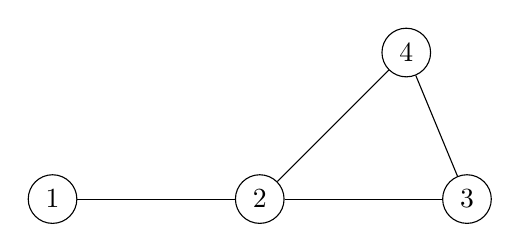
\begin{tikzpicture}[node distance=2cm, auto]
  % Nodes
  \node[circle, draw] (1) {1};
  \node[circle, draw, right=of 1] (2) {2};
  \node[circle, draw, right=of 2] (3) {3};
  \node[circle, draw, above right=of 2] (4) {4};

  % Edges
  \draw (1) -- (2) -- (3);
  \draw (2) -- (4);
  \draw (4) -- (3);
\end{tikzpicture}
\end{center}

The maximum degree $d$ in the graph above is $3$. The graph has a 3-colouring (by using different colours for nodes 1, 2, and 3 and colouring node 4 the same as 1 or 2) and a 4-colouring (by using a different colour for every node), but does not have a 2-colouring.

\begin{questions}

\question[2] For any value of $d$, describe a graph with maximum degree $d$ that can be coloured with two colours.

\ifsolutions\begin{soln}
	Let \(V\) be a vertex set. Add \(v \in V\). Then also add \(v_1, v_2, \dots, v_n\) to \(V\).

	Then for \(v_1, v_2, \dots, v_d\) add \((v, v_i) \in E\) for \(i = 1, 2, \dots, d\).

	Then colour the node \(v\) blue, and colour all other nodes in \(V\) red.

	By construction, the degree of all other nodes that are not \(v\) is \(1\) since it's only connected to \(v\).

	Thus, the degree of \(v\) is the maxmimum degree of the graph, which is \(d\).

	Since no nodes are adjacent except for ones to \(v\). Then the colour red is never shared by adjacent vertices.

	Thus, this graph with maximum degree \(d\) can be coloured with two colours.

\end{soln}
\fi 

\question[2] Consider the following greedy algorithm to find a colouring for a graph:

\begin{quote}
    Order vertices arbitrarily. Colour the first vertex with colour 1. Then choose the next vertex $v$ and colour it with the lowest-numbered colour that has not been used on any previously-coloured vertices adjacent to $v$. If all previously-used colours appear on a vertex adjacent to $v$, introduce a new colour and number it, and assign the new colour to vertex $v$.
\end{quote}

Prove that this algorithm uses at most $d+1$ colours.

\ifsolutions\begin{soln}
	Proof: We provide a proof by induction on the number of nodes, \(n \in \mathbb{N}\), for graph \(G = (V, E)\).

	Base case \(|V| = 1\). The highest degree can be \(d = 0\), since the edge set would be empty.

	Thus, the algorithm uses \(1 = d + 1\) colours to colour the single node and the base case holds.

	Assume for any graph with \(n\) nodes that the algorithm will colour any ordering of nodes using at most \(d + 1\) colours.

	Consider a graph \(G = (V, E)\) with \(|V| = n + 1\) nodes with the highest degree of any node is \(d\).

	Let \(v_1, v_2, \dots, v_n, v_{n+1}\) be any ordering of the nodes. Remove \(v_{n+1}\) from this order, and the graph.

	Denote the deleted graph without \(v_{n+1}\) by \(G'\). Notice the degree of any node in \(G'\) can only decrease.

	Thus, the maximum degree of \(G'\) remains to be \(d\) with the removal of \(v_{n+1}\).

	By assumption, we can colour the ordering \(v_1, v_2, \dots, v_n\) using at most \(d+1\) colours.

	Since \(v_{n+1}\) has degree at most \(d\) then it has at most \(d\) neighbours. Then we add back \(v_{n+1}\).

	The number of colours used to colour its neigbours can be at most \(d\), if each are coloured distinctly.

	Thus, there remains at least \(1\) unique colour to colour \(v_{n+1}\) so that it is a valid colouring.

	In other words, the algorithm uses at most \(d + 1\) colours to colour the ordering \(v_1, v_2, \dots, v_{n+1}\).

	Induction makes the claim holds true for any graph with \(n\) nodes and maximum degree \(d\).


\end{soln}
\fi 

\question[2] Give and briefly explain an example where this algorithm does not produce an optimal colouring (i.e., where it uses more colours than is necessary to colour the graph).

\ifsolutions\begin{soln}
	We consider the graph \(G = (V, E)\) with \(V = \{1, 2, 3, 4\}\) and \(E = \{(1, 4), (4, 3), (3, 2)\}\).

	\begin{center}
		\begin{tikzpicture}[node distance=2cm, auto]
			% Nodes
			\node[circle, draw, above  right = of 3] (1) {1};
			\node[circle, draw, right=of 1] (2) {2};
			\node[circle, draw, right=of 2] (3) {3};
			\node[circle, draw, above right=of 2] (4) {4};

			% Edges
			\draw (1) -- (4) -- (3) -- (2);
		\end{tikzpicture}
	\end{center}

	This graph can be coloured with three colours. Namely we can assign \(A = \{1, 3\}\) \(B = \{2, 4\}\).

	We see that no edges are shared between any vertices in \(A, B\) so this is a valid colouring.

	Now consider the ordering \(1, 2, 3, 4\). We first colour \(1\) blue. And then we consider \(2\).

	There is no edge between \(1, 2\) so we colour \(2\) blue and consider \(3\).

	So, its adjacent vertices have been coloured with blue, then we introduce a new colour for it red.

	Now we finally consider \(4\), its neighbours have been coloured with both red and green, so we must introduce a new colour for it purple.

	We have thus coloured this graph using three colours through the greedy algorithm when we could have used two.


\end{soln}
\fi 

\question[5] Now, assume that there is at least one vertex $v$ in $V$ with degree \textbf{less than} $d$.  Design a greedy algorithm that will colour vertices of $G$ with at most $d$ colours. You should proceed by first \textbf{ordering the vertices} in some way, and then assigning colours using the colouring strategy in question 4.2. You should explain why your algorithm uses no more than $d$ colours.

\ifsolutions\begin{soln}
	fuck you
\end{soln}
\fi 

\end{questions}
	\ifsolutions\else\newpage\fi

        \section{Constrained Shortest Paths}
A  company is leasing communication bandwidth from a national telecom provider to establish  a new connection between its office in Vancouver and its office in Newark.

The telecom provider's network is represented by a graph $G=(V,E)$ and each edge $(u,v)$ has an advertised price $p(u,v)$.  In addition, each edge
has a transit delay $d(u,v)$ due to node equipment. Suppose a new connection is to be established between two given nodes $s,t \in V$ and we require that the total delay between the two nodes be no more than $D$. Assume that all prices and delays are greater than 0. The company would therefore like to find the cheapest $st$-path which obeys  this constraint. In other words, the problem to solve is:
\[
	\min_{\mbox{$P$ an $st$-path}}  p(P) \textrm{ such that } d(P)\leq D
\]

Here $p(P)$ denotes the price of the path $P$ -- that is $\sum_{(u,v) \in P} p(u,v)$ -- and $d(P)$ denotes the total delay of the path $P$ -- that is, $\sum_{(u,v) \in P} d(u,v)$.


\begin{questions}
	\question[5] For each $v \in V$, define
	$P(\delta,v)$ to be  the minimum cost of a path from $s$ to $v$ with total communication delay at most $\delta$. Write a recurrence to define $P(\delta, v)$.

	\ifsolutions\begin{soln}
	Consider the instance:

	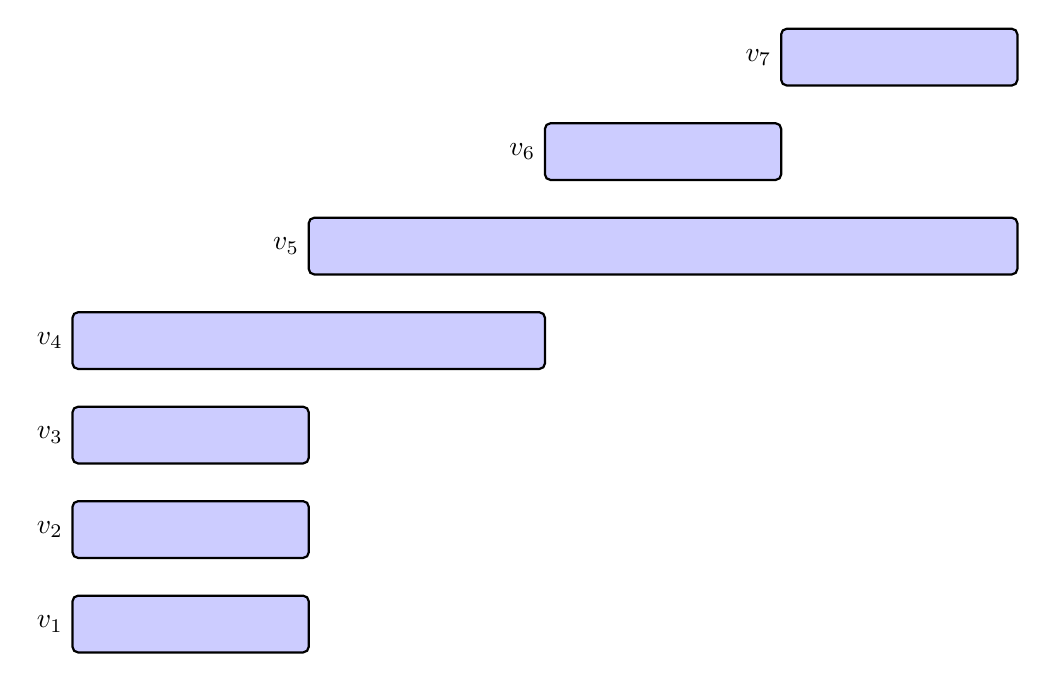
\begin{tikzpicture}[xscale=3, yscale=1.2]

		% Draw each interval as a bar
		\foreach \name/\start/\end/\y in {
				v_1/0/1/1,
				v_2/0/1/2,
				v_3/0/1/3,
				v_4/0/2/4,
				v_5/1/4/5,
				v_6/2/3/6,
				v_7/3/4/7
			} {
				\draw[thick, fill=blue!20, rounded corners=2pt] (\start,\y) rectangle (\end,\y+0.6);
				\node[left] at (\start,\y+0.3) {\(\name\)};
			}

	\end{tikzpicture}


	We see that in the proposed greedy algorithm that \(v_4\) intersects with the most amount of shifts, \(4\).

	After removing all intersections, only \(v_6, v_7\) remains, since those two are disjoint, the greedy algorithm returns volunteers \(v_4, v_6, v_7\) as its best solution.

	But notice that, by taking volunteers the two \(v_1, v_5\) we sufficiently cover all shifts in the set, thus this greedy algorithm is not optimal on all instances.

\end{soln}
\fi

	\begin{soln}
		First, define a base case, the path from \(s\) to itself will have cost zero, so long as the delay is non-negative.

		If delay is less then zero, we will give it a cost of ininfity, since delays are assumed to be non-negative.

		For the other cases, consider the last node in the path and the node that precedes it, denote it by \(u\).

		If \(u\) is going to precede it, then the path from \(s\) to \(u\) should have delay at most \(\delta - d(u, v)\).

		Since we want the minimized cost path, then \(P(\delta, v) = \min_{(u, v) \in E} (P(\delta - d(u, v), u) + p(u, v))\).

		\[
			P(\delta, v) = \begin{cases}
				0                                                      & \text{if } s = v \text{ and } \delta \geq 0 \\
				\infty                                                 & \text{ if } \delta < 0                      \\
				\min_{(u, v) \in E} (P(\delta - d(u, v), u) + p(u, v)) & \text{ otherwise }
			\end{cases}
		\]

	\end{soln}

	\question[7] Give a recursive memoized algorithm to solve for $P(D,v)$ for a given maximum delay $D$ and node $v$.

	\ifsolutions\begin{soln}
	Sort the shifts in terms of ascending order by finish time, for any ties, place first the earliest start time.

	Choose the first shift in the ordered list, and add it to our solution set.

	Then delete any intersecting shifts to that shift and remove that shift itself from the ordered list.

	Continue to the next shift in the ordered list and repeat the previous steps until the list is empty.
\end{soln}

\fi

	\begin{soln}
		Assume that all relevant functions and arrays are defined.

		I.e. weight functions for delays \(d\), cost weight functions \(p\), adjacency lists, edge lists.

		\begin{algorithmic}[1]
			\Procedure{Find-Best-Path-Wrapper}{$D, v$}
			\State Define $P[(\delta, u)] = $ min cost to reach node $u$ from $s$ with delay at most $\delta$ using a dictionary
			\State \Return Find-Best-Path($D, v, P$)
			\EndProcedure
		\end{algorithmic}

		\newpage

		\begin{algorithmic}[1]
			\Procedure{Find-Best-Path}{$\delta, u, P$}
			\If {$s = u$ and $\delta \geq 0$}
			\State \Return $0$
			\EndIf
			\If {$\delta < 0$}
			\State \Return $\infty$
			\EndIf
			\If{$P[(\delta, u)] = None$}
			\State $P[(\delta, u)] = \min_{(u', u) \in E}(\text{Find-Best-Path}(\delta - d(u', u), u', P) + p(u', u))$
			\EndIf
			\State \Return $P[(\delta, u)]$
			\EndProcedure
		\end{algorithmic}

	\end{soln}




\end{questions}

	\ifsolutions\else\newpage\fi
\end{document}